% Section content template for individual Educative lessons
% This file contains the actual content for a specific section
% Generated from Educative API section content

% Section: Use Case Diagram for the Library Management System
% Section ID: 6616873252945920
% Section Slug: use-case-diagram-for-the-library-management-system
% Generated: 2025-12-11T15:12:16.762994

Let's build the use case diagram for the library management system and understand the relationships between its main actors, system functions, and user interactions. First , we will define the different elements of our library, followed by the complete use case diagram of the system.

\subsection{System}\label{0ubFJ51N6k4NDPk2NKe6F}
\\
Our system is the library management system. It manages the library's catalog, member accounts, book transactions, and notifications.

\subsection{Actors}\label{xx5ay0GYZD-qjnudajTgv}
\\
Next, we will define the main actors of our library management system.

\subsubsection{Primary actors}\label{rVsk3lbKBYgP6Yg2os4pZ}

\begin{itemize}
\item
\protect\phantomsection\label{cXZdpFr7k5QCPcDIdJRwi}
\textbf{Member:} A library member who can search, reserve, borrow, renew, or return books, pay fines, and request membership cancellation.
\item
\protect\phantomsection\label{7ewneLUTbIder7qY-FrpB}
\textbf{Librarian:} The administrator responsible for managing books and book items, issuing and returning books, handling reservations, managing member accounts, and overseeing fines.
\end{itemize}

\subsubsection{Secondary actors}\label{Yb9cGDFw2Szq6JwmpEivm}

\begin{itemize}
\item
\protect\phantomsection\label{jMcrrvs2GYW-aLCCapt0G}
\textbf{System:} It can send alerts related to reservations and late returns of books.
\end{itemize}

\subsection{Use cases}\label{6QmDNyPmjH9OLYt8xMCg1}
\\
In this section, we will define the library's use cases. We have listed them according to their interactions with a particular actor.
\begin{quote}
\textbf{Note:} Some use cases will occur multiple times because they are shared among different actors in the system.
\end{quote}
\subsubsection{Member}\label{poqsLui6wHPhnv2lhyyva}

\begin{itemize}
\item
\protect\phantomsection\label{Yj2VSP5PW1aLRw9oVqfMn}
\textbf{Login/Logout:} To securely access or exit their member account and access library services.
\item
\protect\phantomsection\label{7JRYMEALF8zzrYk7yWJYE}
\textbf{Register/Update account:} To create a new membership account or update personal and contact information.
\item
\protect\phantomsection\label{04w6eGxteMWC9soKIKdbr}
\textbf{Cancel membership:} To voluntarily request termination of their library membership.
\item
\protect\phantomsection\label{GtB-K_UxQjr70fCu0wyvn}
\textbf{View account:} To review their own account details, borrowing history, current checkouts, reservations, and fines.
\item
\protect\phantomsection\label{hAA-jR3Y_4x_r5xDmFd8y}
\textbf{Search catalog:} Search the library catalog for books or resources by title, author, subject, or publication date.
\item
\protect\phantomsection\label{_r4p2PWbgay-RVK5m9a6a}
\textbf{Reserve book:} To place a hold on a currently checked-out book, ensuring it can be borrowed when it becomes available.
\item
\protect\phantomsection\label{OyWTiRFAu6rZsNPt667W0}
\textbf{Checkout book:} To complete the process of borrowing a book, either directly or by following a successful reservation.
\item
\protect\phantomsection\label{uUVinSWKSKx63Cs-XXS2z}
\textbf{Renew book:} To request an extension for the borrowing period of a currently issued book.
\item
\protect\phantomsection\label{cIUkq3O_k78-3ua0Lbaw7}
\textbf{Return book:} To return a borrowed book to the library, update the system, and potentially make it available for other members.
\item
\protect\phantomsection\label{Yw3IjE09-viL4nbrmlUMU}
\textbf{Remove reservation:} To cancel a previously placed hold on a book.
\item
\protect\phantomsection\label{Q0JRrLvGH-jlNvZ2klCWt}
\textbf{Pay fine:} To settle any outstanding fines incurred due to overdue book returns or other violations, allowing the member to maintain good standing.
\end{itemize}

\subsubsection{Librarian}\label{8mwX3gsZWSsW-gIvgCd-E}

\begin{itemize}
\item
\protect\phantomsection\label{PuHAINXkOLU4W-w1aaXOQ}
\textbf{Login/Logout:} To securely access or exit the librarian account and manage system resources.
\item
\protect\phantomsection\label{zFBoHDyK-UwvXqaMsmdk6}
\textbf{Register/Update account:} To register a new library member by collecting and saving their details in the system, or modify a member's personal details or membership status.
\item
\protect\phantomsection\label{CPzU4hfiMsc7WggwxDKH0}
\textbf{Cancel membership:} To terminate the library membership of a member and deactivate their account.
\item
\protect\phantomsection\label{1z0YHRqgD6DIZYxb2LL4p}
\textbf{View account:} To access and review a library member's account details and history.
\item
\protect\phantomsection\label{sf7Qsw03sutXh8CkjcPPg}
\textbf{Issue library card:} To create and assign a unique one to a new member during registration, enabling them to borrow books and access other library services.
\item
\protect\phantomsection\label{udX0jHDgNPNaPzIXTQCFJ}
\textbf{Add book:} To add a new book entry to the library's catalog, including essential metadata such as author, ISBN, etc.
\item
\protect\phantomsection\label{CFjrrtxtBN3H2hgGtGCx7}
\textbf{Edit book:} To update the information of an existing book in the library catalog.
\item
\protect\phantomsection\label{MxBd-qBOMxX5MOynyeRxQ}
\textbf{Remove book:} To delete a book record from the library catalog, typically if it is no longer part of the library's collection.
\item
\protect\phantomsection\label{qIfGrHvMbJufw7kbMDtd3}
\textbf{Add book item:} To add a physical copy of a book to the library's inventory (e.g., when purchasing additional copies).
\item
\protect\phantomsection\label{bkyKCC5m83ZPmqpsQDNT-}
\textbf{Edit book item:} To update a specific physical book copy's details (such as rack location).
\item
\protect\phantomsection\label{LjUkbVd41-jhQ9TYOFwai}
\textbf{Remove book item:} To delete a specific book copy from the inventory.
\item
\protect\phantomsection\label{wzLMk-joSmW2q38IUjdO-}
\textbf{Issue book:} To lend a book item to a library member, recording the issuance in the system.
\item
\protect\phantomsection\label{IYSxY3XYk95Z021uV7t_G}
\textbf{Renew book:} To extend the borrowing period for a book already issued to a member, per library policy.
\item
\protect\phantomsection\label{Xch7XVzuG1MJ6t4lKXXfn}
\textbf{Update catalog:} To comprehensively manage the library catalog by adding, editing, or removing books or book items.
\item
\protect\phantomsection\label{dyt_mHzk8Kyo9jyOa1RHX}
\textbf{Remove reservation:} To cancel a member's book reservation, make the book available to others.
\end{itemize}

\subsubsection{Library management system}\label{PwSssY8oFBZCleQTscbEu}

\begin{itemize}
\item
\protect\phantomsection\label{DF6DoiVDIOl_ApxkHVnJY}
\textbf{Calculate fine:} To automatically determine the fine amount for overdue books based on the return date and the library's fine policy.
\item
\protect\phantomsection\label{N0JG4CuCdaFmauP4Rl_XQ}
\textbf{Send overdue notification:} To send alerts to members when the return due date for a borrowed book has passed, prompting action.
\item
\protect\phantomsection\label{W7H8N2HewEO5pwWJP1Ntr}
\textbf{Send reservation available notification:} To inform members when a previously reserved book becomes available for borrowing or checkout.
\item
\protect\phantomsection\label{XWpYO4g1N9PUUjKtGI7zw}
\textbf{Send reservation canceled notification:} To notify members when their reservation for a book has been canceled.
\end{itemize}

\subsection{Relationships}\label{iFnbUTv-9Y2NrB6jSIH9G}
\\
This section describes the relationships between and among actors and their use cases.

\subsubsection{Generalization}\label{Io6fG83UVen8flYWngd4r}
\\
\emph{Search catalog} is a generalized use case. Members can search by different attributes. Specialized use cases include:

\begin{itemize}
\item
\protect\phantomsection\label{eTIWGam3Y_SvFAd2yDUsg}
\textbf{Search by title}
\item
\protect\phantomsection\label{DOjJ2ZJ8KzfpZ4-Lp5pKy}
\textbf{Search by author}
\item
\protect\phantomsection\label{BvvgGjXjQPn5ayYfyHK5h}
\textbf{Search by subject}
\item
\protect\phantomsection\label{zIMBnCIVscvDgi5ZbDcrV}
\textbf{Search by publication date}
\end{itemize}
\\
This means that ``search catalog'' generalizes the more specific search methods.

\subsubsection{Associations}\label{AZuKozZoPAwRed1Jxg87-}
\\
The table below shows the association relationship between actors and their use cases.

\begin{center}
\begin{tabular}{|p{0.3\linewidth}|p{0.3\linewidth}|p{0.3\linewidth}|}
\hline
\textbf{Librarian} & \textbf{Member} & \textbf{Library Management System} \\
\hline
Log in/Log out & Log in/Log out & Calculate fine \\
\hline
Register/Update account & Register/Update account & Send overdue notification \\
\hline
Cancel membership & Cancel membership & Send reservation available notification \\
\hline
View account & View account & Send reservation canceled notification \\
\hline
Issue library card & Search catalog & Add book \\
\hline
Check out book & Reserve book & Edit book \\
\hline
Renew book & Add book item & Remove book \\
\hline
Return book & Edit book item & Remove reservation \\
\hline
Pay fine & Issue book & Renew book \\
\hline
Update catalog & Remove reservation & Remove book item \\
\hline
\end{tabular}
\end{center}


\subsubsection{Include}\label{9wfm14MznDdHSvsYcbvJC}
\\
When a librarian adds, edits, or removes a book from the catalog, they must also manage the associated book items (physical copies). These steps are best represented using ``include'' relationships in a use case diagram:

\begin{itemize}
\item
\protect\phantomsection\label{Kp1b_tXwwB7N6PFJZB8ta}
\textbf{Add book, Edit book, and Remove book} use cases all include the \textbf{Add book item, Edit book item, and Remove book item} use cases, respectively.
\item
\protect\phantomsection\label{Cdn61g_CTdSxmLGDIRZe1}
\textbf{Add book item}, \textbf{Edit book item}, and \textbf{Remove book item} each include \textbf{Update catalog}, ensuring the catalog stays consistent after each change.
\end{itemize}
\\
When registering a new member, the librarian must issue a library card to enable borrowing privileges:

\begin{itemize}
\item
\protect\phantomsection\label{J0j6HamzyMP4hY_dfBzi9}
The \textbf{Register new account} use case includes the \textbf{Issue library card} use case.
\end{itemize}
\\
When issuing a book to a member, the librarian or system completes the checkout process:

\begin{itemize}
\item
\protect\phantomsection\label{-cLIMzsQzIFtxcCFaz9_o}
The \textbf{Issue book} use case includes the \textbf{Checkout book} use case.
\end{itemize}
\\
During checkout, if the member had reserved the book, the system removes the reservation:

\begin{itemize}
\item
\protect\phantomsection\label{fLZSJh_UKoYoJVSpxdDmc}
The \textbf{Checkout book} use case includes the \textbf{Remove reservation} use case.
\end{itemize}
\\
For overdue books, when a member returns a book late, the system automatically calculates the fine:

\begin{itemize}
\item
\protect\phantomsection\label{-7sDUatbnsmdNQEtkQjkJ}
The \textbf{Return book} use case includes the \textbf{Calculate fine} use case.
\end{itemize}

\subsubsection{Extend}\label{efas7YpdDQm-uaHeKwt27}
\\
When a member returns a book, additional steps may be required if certain conditions are met. These conditional actions are best represented using \textbf{«extend»} relationships in a use case diagram:

\begin{itemize}
\item
\protect\phantomsection\label{hHJO-Z9YI0oEzwTA60B0N}
The \textbf{Pay fine} use case extends the \textbf{Return book} use case if the book is returned after the due date.
\end{itemize}
\\
For the reservation process, if a reserved book becomes available, the system will notify the member:

\begin{itemize}
\item
\protect\phantomsection\label{FHaA0KLUlcGlo50OZcGCd}
The \textbf{Send reservation available notification} use case extends the \textbf{Reserve book} use case when the reserved book becomes available.
\end{itemize}
\\
When a member cancels a reservation, the system sends a notification:

\begin{itemize}
\item
\protect\phantomsection\label{eCigDDMlAGjbS1CMLKsI3}
The \textbf{Send reservation canceled notification} use case extends the \textbf{Remove reservation} use case.
\end{itemize}

\subsection{Use case diagram}\label{BVnN1lviKoC09pk0JZoA6}
\\
Here is the use case diagram of the library management system:

\begin{figure}[htbp]
 \centering
 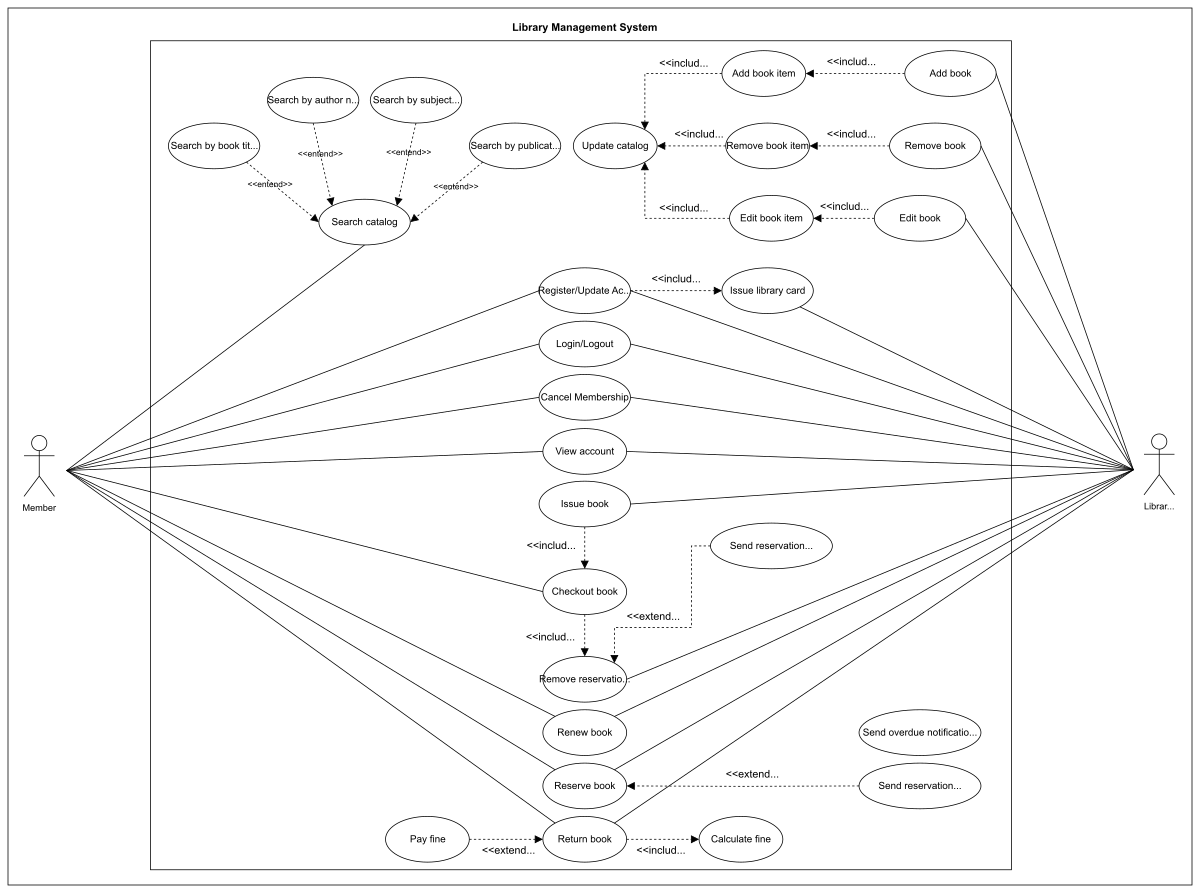
\includegraphics[width=0.5\textwidth]{Images/chapter_9/section_6616873252945920/5507241882812416.png}
 \caption{Use case diagram of the library management system}
\end{figure}

In the next lesson, we will discuss the class diagram with a detailed explanation of all classes and their relationship with each other.

% End of section content